\documentclass[lettersize,journal]{IEEEtran}
\usepackage{amsmath,amsfonts}
\usepackage{algorithmic}
\usepackage{algorithm}
\usepackage{array}
\usepackage[caption=false,font=normalsize,labelfont=sf,textfont=sf]{subfig}
\usepackage{textcomp}
\usepackage{stfloats}
\usepackage{url}
\usepackage{verbatim}
\usepackage{graphicx}
\usepackage{cite}
\usepackage{hyperref}
\usepackage{booktabs}
\usepackage{multirow}
\graphicspath{{figures/}}
\hyphenation{op-tical net-works semi-conduc-tor IEEE-Xplore Vin-Fast}

\begin{document}

\title{Electric Vehicle Price Prediction in the Vietnamese Market:\\ A Web-Scraped Dataset with LLM-Assisted Feature Extraction}

\author{Anh~D.~D.~Hoang, Khang~H.~Tran, Anh~N.~Vu, ~and~Nam~N.~Trinh
\thanks{The authors are with Information Technology Specialization, FPT University, Hanoi, Vietnam.}
\thanks{Manuscript prepared March 2026.}}

%\markboth{[Journal/Conference Name],~Vol.~X, No.~Y, Month~2026}%
\markboth{AIL301m, March~2026}%
{Anh~D.~D.~Hoang \MakeLowercase{\textit{et al.}}: EV Price Prediction in Vietnam}

\maketitle

% ============================================================================
\begin{abstract}
The rapid growth of the electric vehicle (EV) market in Vietnam has created
demand for automated price estimation tools, yet no publicly available
structured dataset exists for Vietnamese EV listings. This paper presents an
end-to-end pipeline for EV price prediction, from web scraping of four major
Vietnamese car marketplaces to regression modeling. We introduce a two-stage
LLM-assisted feature extraction approach using local (Qwen~2.5 3B) and
cloud-based (GPT-5-nano) models to parse unstructured Vietnamese car listings
into structured features. Through systematic data quality analysis, we
identify and correct three critical issues---a 10$\times$ price inflation
affecting 40\% of records, systematic brand-level pricing errors, and 22.2\%
duplicate contamination causing test--train leakage---reducing RMSE from
1.02~billion~VND (artificially deflated by leakage) to 332~million~VND
(honest evaluation). We benchmark four regression models (Ridge, SVR, Random
Forest, XGBoost) across price segments and find that Random Forest achieves
the best overall performance ($R^2 = 0.725$, RMSE~$= 332$M~VND), with
practical accuracy for budget and mid-range segments comprising 92\% of
our test records. Our analysis highlights that data quality remediation contributes
more to prediction accuracy than model selection in this domain.
\end{abstract}

\begin{IEEEkeywords}
Electric vehicle, price prediction, web scraping, large language model,
feature extraction, data quality, regression, Vietnamese market.
\end{IEEEkeywords}

% ============================================================================
\section{Introduction}
\IEEEPARstart{V}{ietnam's} electric vehicle market has experienced
unprecedented growth since VinFast, the country's first domestic automaker,
began mass-producing EVs in 2022. With the Vietnamese government's roadmap to
phase out internal combustion engine vehicles by 2040~\cite{vn_ev_policy} and
an influx of Chinese EV imports (BYD, Wuling, Geely), the market is expanding
rapidly. However, unlike mature markets in the US and Europe where structured
pricing databases and valuation tools (e.g., Kelley Blue Book, AutoTrader)
exist, Vietnam's EV market lacks any publicly available structured dataset or
automated pricing tool.

Existing literature on car price prediction predominantly relies on clean,
structured datasets sourced from dealer APIs or curated platforms such as
Kaggle~\cite{vw_price, gegic2019}. These studies typically focus on
established Western markets where listing data follows standardized schemas.
The Vietnamese automotive marketplace presents fundamentally different
challenges: listings are unstructured, written in Vietnamese with
inconsistent formatting, distributed across multiple platforms with
incompatible schemas, and subject to systematic data quality issues that are
absent from curated datasets.

Recent advances in large language models (LLMs) offer a promising approach
to parsing unstructured listings into structured features. However, LLM
extraction introduces its own quality concerns, including hallucinated
values and systematic unit errors that propagate through the pipeline.

This paper makes four contributions:
\begin{enumerate}
    \item We construct the first Vietnamese EV dataset by scraping and
    harmonizing listings from four major car marketplaces, yielding 4,166 raw
    records with a 20-column unified schema.
    \item We design a two-stage LLM-assisted feature extraction pipeline
    using a local 3B-parameter model (Qwen~2.5) with cloud-based
    verification (GPT-5-nano), incorporating auto-retry and Pydantic-based
    validation.
    \item We conduct systematic data quality analysis that identifies three
    critical issues---source-level price inflation, brand-level systematic
    error, and duplicate-induced test--train leakage---and demonstrate that
    correcting these issues reduces RMSE by 67\%, from 1.02B to 332M~VND.
    \item We provide segment-specific evaluation showing that the model
    achieves practical accuracy (RMSE $< 100$M~VND) for budget and mid-range
    segments, which comprise 92\% of our test records.
\end{enumerate}

% ============================================================================
\section{Related Work}

\subsection{Car Price Prediction}
Hedonic pricing models have long been used to estimate vehicle values based
on observable characteristics~\cite{hedonic_pricing}. More recently, machine
learning approaches have shown improved accuracy. Gegic et al.~\cite{gegic2019}
compared multiple regression models on a Bosnian used-car dataset and found
that Random Forest outperformed linear models. Pal et al.~\cite{pal2018}
applied Lasso and Random Forest to Indian car prices, achieving $R^2 > 0.90$
on a clean dealer dataset. Pudaruth~\cite{pudaruth2014} demonstrated that
ensemble methods consistently outperform single models for used car valuation
in Mauritius.

A common limitation of these studies is their reliance on pre-cleaned,
single-source datasets. Our work differs by constructing a multi-source
dataset from heterogeneous web platforms and explicitly addressing the data
quality challenges that arise from this approach.

\subsection{Web Scraping for Dataset Construction}
Web scraping has been widely adopted for constructing research datasets in
domains where structured data is unavailable~\cite{mitchell_scraping}. In the
automotive domain, Lessmann et al.~\cite{lessmann2019} scraped European car
listings to study depreciation curves. However, the challenges of scraping
Vietnamese-language marketplaces---including encoding issues, inconsistent
pricing units, and platform-specific data formats---remain underexplored.

\subsection{LLM-Based Information Extraction}
The application of LLMs for structured information extraction from
unstructured text has gained traction~\cite{wei2023}. Recent work has
demonstrated that even small language models (3B--7B parameters) can
effectively extract structured data when combined with appropriate prompting
and validation strategies~\cite{ollama2024}. Our pipeline extends this
approach with a two-stage architecture and domain-specific guardrails.

% ============================================================================
\section{Data Collection}

\subsection{Source Websites}
We scraped EV listings from four Vietnamese car marketplace websites, each
offering different coverage, data quality, and listing formats. Table~\ref{tab:sources}
summarizes the source characteristics.

\begin{table}[!t]
\caption{Data Source Characteristics\label{tab:sources}}
\centering
\begin{tabular}{lllr}
\toprule
\textbf{Website} & \textbf{Method} & \textbf{Coverage} & \textbf{Records} \\
\midrule
bonbanh.com & BeautifulSoup & Multi-brand & 1,493 \\
chotot.com & Scrapy & Multi-brand & 1,666 \\
xevinfastluot.com & Selenium & VinFast only & 279 \\
otodien.vn & BeautifulSoup & Multi-brand & 728 \\
\midrule
\multicolumn{3}{l}{\textbf{Total (merged)}} & \textbf{4,166} \\
\bottomrule
\end{tabular}
\end{table}

Each website required a different scraping strategy due to varying levels of
JavaScript rendering and anti-bot measures. bonbanh.com and otodien.vn serve
static HTML and were scraped using BeautifulSoup~\cite{bs4}. chotot.com
uses dynamic loading and was handled with Scrapy~\cite{scrapy} and custom
middleware. xevinfastluot.com, a VinFast-specialized dealer portal, required
Selenium~\cite{selenium} for browser-based interaction.

\subsection{Schema Harmonization}
The four sources use incompatible listing schemas. We designed a unified
20-column schema covering: identification (id, brand, base\_model,
model\_mode), specifications (year, mileage\_km, body\_type, seats, doors,
drivetrain, origin), condition indicators (condition, has\_aftermarket\_mods,
exterior\_color), metadata (city, seller\_name, post\_date, website), and the
target variable (price\_vnd). Records from all four sources were mapped to
this schema using source-specific transformation scripts.

Fig.~\ref{fig:records_per_source} shows the distribution of records across
sources after harmonization.

\begin{figure}[!t]
\centering
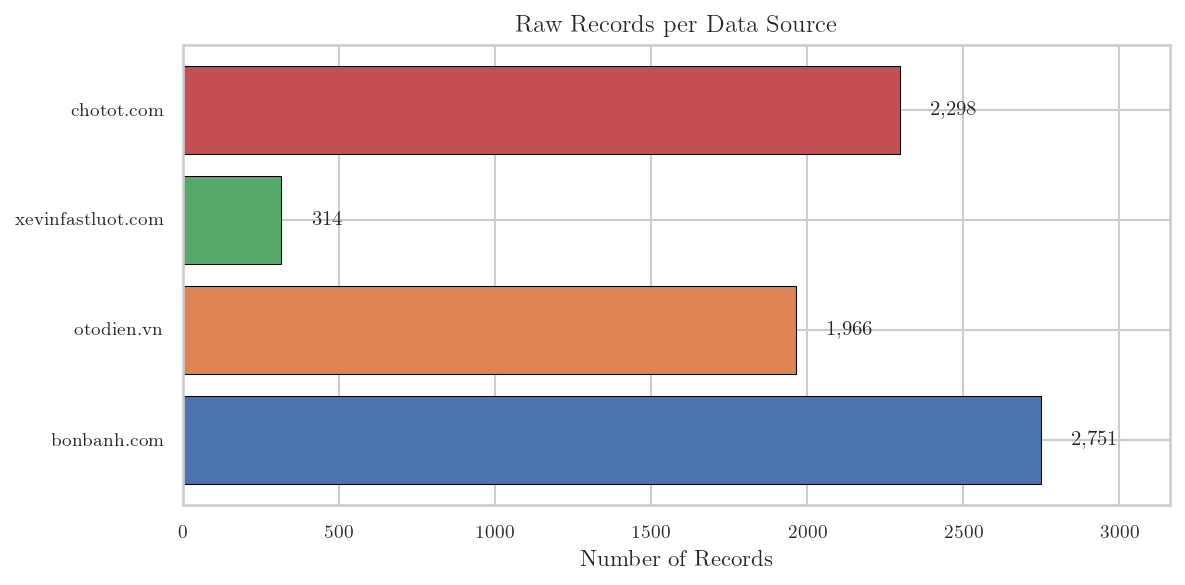
\includegraphics[width=\columnwidth]{records_per_source}
\caption{Distribution of records across the four data sources.}
\label{fig:records_per_source}
\end{figure}

% ============================================================================
\section{LLM-Assisted Feature Extraction}

Raw car listings from Vietnamese websites contain critical pricing features
(trim level, battery capacity, drivetrain configuration) embedded in
unstructured Vietnamese text. Traditional regex-based extraction fails on the
diverse naming conventions across platforms.

\subsection{Two-Stage Pipeline}
We designed a two-stage extraction pipeline:
\begin{enumerate}
    \item \textbf{Local extraction (Qwen~2.5 3B):} Each listing's raw text
    is processed by a locally-hosted Qwen~2.5 3B model via Ollama~\cite{ollama2024}.
    The model extracts structured fields (brand, model, trim, year,
    condition, specifications) using a zero-shot prompt with JSON output
    constraints. A Pydantic schema validates the output, and failed
    extractions trigger automatic retry with a rephrased prompt (up to 3
    attempts).
    \item \textbf{Cloud verification (GPT-5-nano):} Records where the local
    model produced low-confidence or inconsistent results are batch-processed
    through OpenAI's GPT-5-nano API for verification and correction.
\end{enumerate}

\subsection{Extraction Quality}
The two-stage approach achieved high fill rates for core fields: brand
(99.3\%), base\_model (98.7\%), year (98.3\%), and price (100\%). The primary
failure mode was trim-level extraction (model\_mode), where the local model
occasionally hallucinated non-existent trim names for non-VinFast brands.

% ============================================================================
\section{Data Quality Analysis}

Prior to the quality analysis described in this section, a rule-based
preprocessing step (\texttt{preprocess\_rule\_based.py}) reduced the 4,166
merged records to 3,992 by removing non-EV (ICE) listings, records with
missing or structurally invalid prices, and malformed entries. The remaining
3,992 records then underwent systematic data quality analysis, which
revealed three critical issues.



\subsection{chotot.com 10$\times$ Price Inflation}
Cross-source price comparison revealed that listings from chotot.com
exhibited prices approximately 10$\times$ higher than equivalent listings on
other platforms. For example, a VinFast VF5 Plus 2024 was listed at
3.99B~VND on chotot.com versus 399M~VND on bonbanh.com. This affected
1,666 records (40.0\% of the merged dataset) and was traced to
chotot.com storing listing prices in units of 1{,}000~VND, which were
ingested as raw VND values during scraping and harmonization.

The correction was straightforward: dividing all chotot.com prices by 10.
Fig.~\ref{fig:chotot_price} illustrates the price discrepancy before
correction.

\begin{figure*}[!t]
\centering
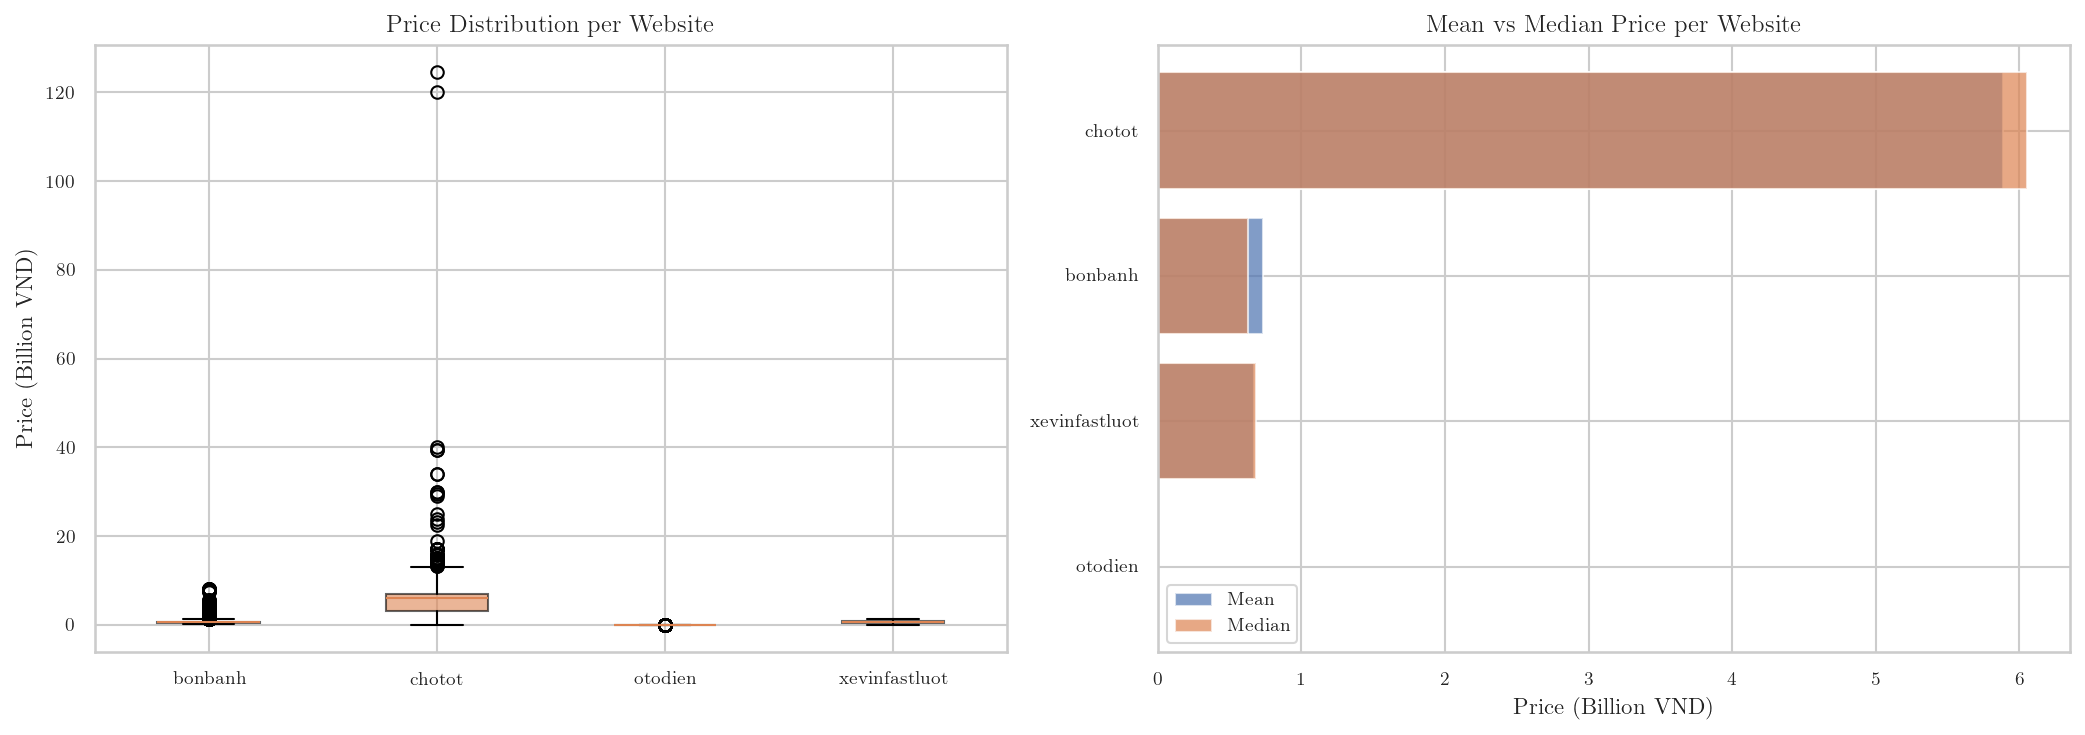
\includegraphics[width=\textwidth]{chotot_price_comparison}
\caption{Price comparison between chotot.com and other sources for the same
vehicle models, showing systematic 10$\times$ inflation.}
\label{fig:chotot_price}
\end{figure*}

\subsection{BYD Systematic Pricing Error}
All 90 BYD-brand records (2.3\% of the dataset) exhibited prices
approximately 10$\times$ higher than actual market values. Unlike the
chotot.com issue, this error was brand-specific and appeared across all
sources. Because every BYD record was affected, no within-brand correction
was possible. Despite representing only 2.3\% of records, a simulation shows BYD would
account for approximately 56\% of total weighted prediction error if
retained---with a per-record MAE of 4.914B~VND versus 89.5M~VND for
non-BYD records under the best-performing model. We removed all BYD records
from the training dataset.

Fig.~\ref{fig:byd_removal} shows the price distribution comparison between
BYD and non-BYD records.

\begin{figure}[!t]
\centering
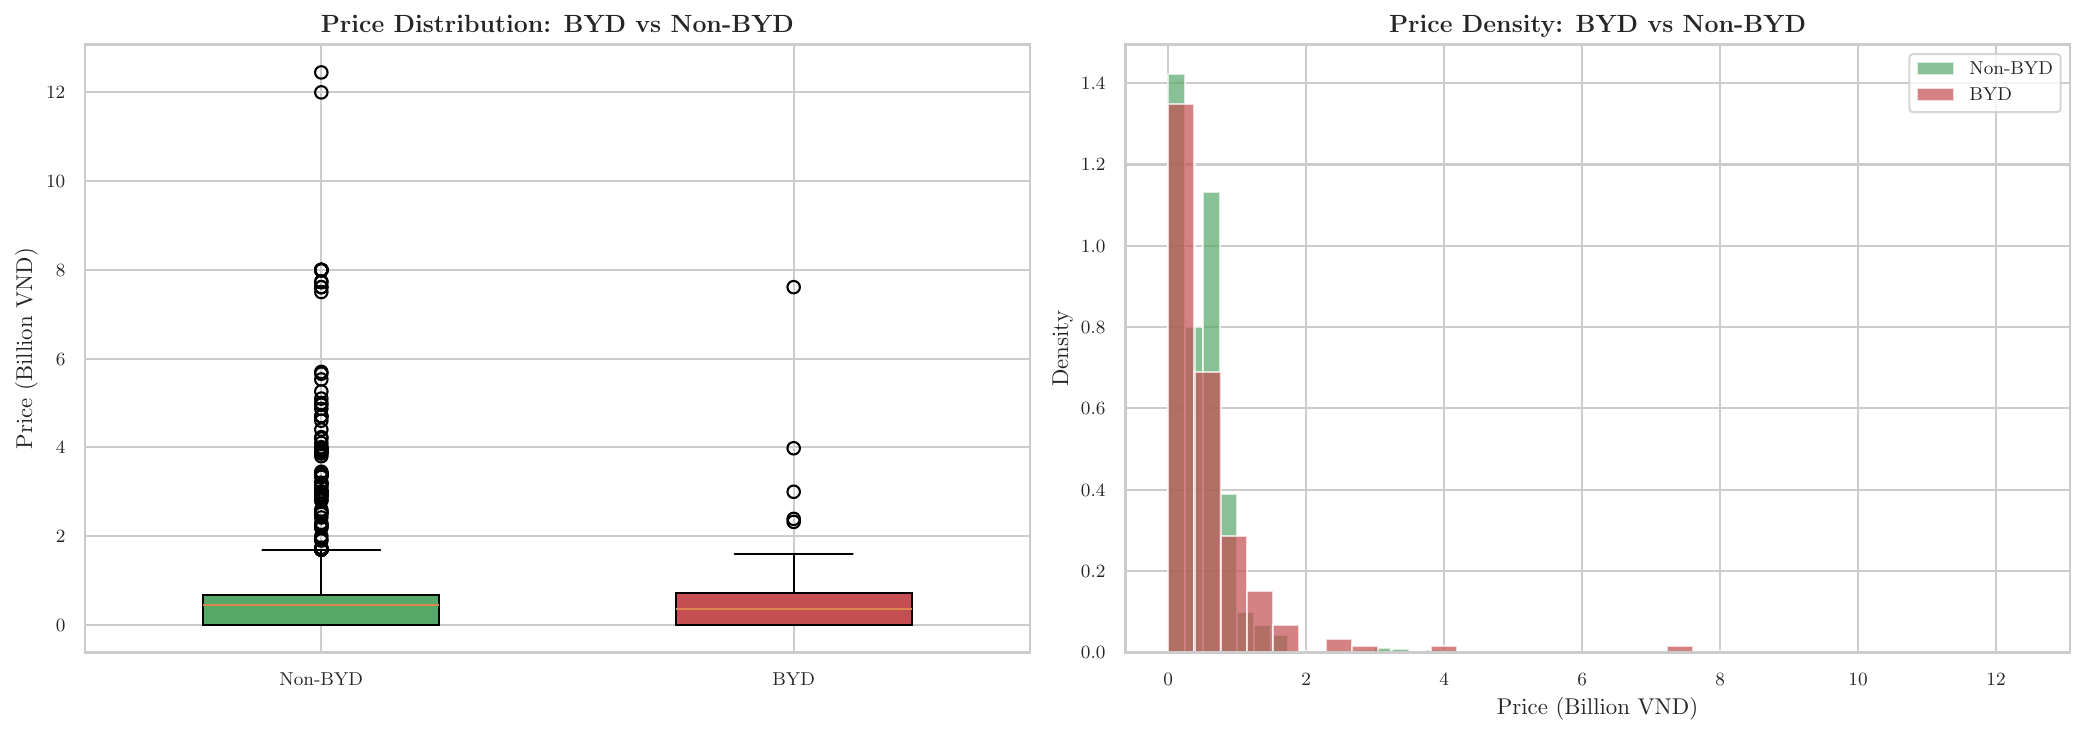
\includegraphics[width=\columnwidth]{byd_removal}
\caption{Price distribution: BYD (all records 10$\times$ inflated) versus
non-BYD brands.}
\label{fig:byd_removal}
\end{figure}

\subsection{Duplicate Contamination and Test--Train Leakage}
Deduplication analysis on the key tuple (brand, base\_model, model\_mode,
year, price\_vnd, condition, mileage\_km) revealed that 887 records (22.2\%
after price correction) were exact duplicates. The most extreme case---a
VinFast VF9 2025 at 12.29B~VND---appeared 23 times.

When duplicates span both training and test sets, the model effectively
memorizes rather than generalizes, producing artificially inflated
performance metrics. Before deduplication, the apparent best $R^2$ was 0.787;
after proper deduplication, the honest $R^2$ was 0.725---a 7.9\% reduction
revealing the extent of leakage.

Fig.~\ref{fig:dedup} and Fig.~\ref{fig:before_after} illustrate the
deduplication impact.

\begin{figure}[!t]
\centering
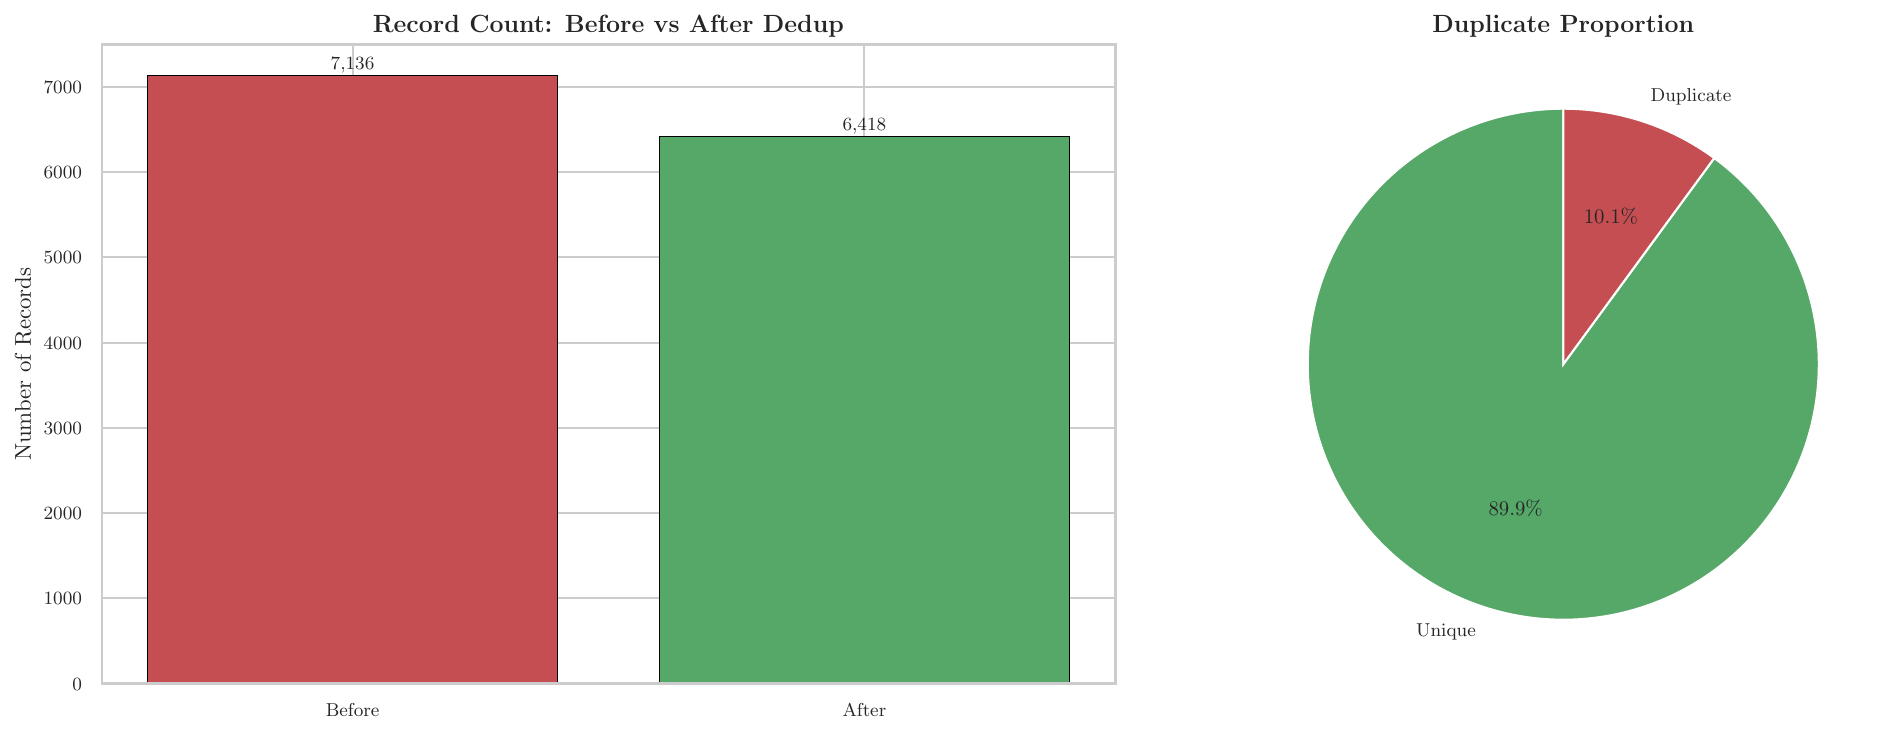
\includegraphics[width=\columnwidth]{dedup_analysis}
\caption{Record counts before and after deduplication.}
\label{fig:dedup}
\end{figure}

\begin{figure*}[!t]
\centering
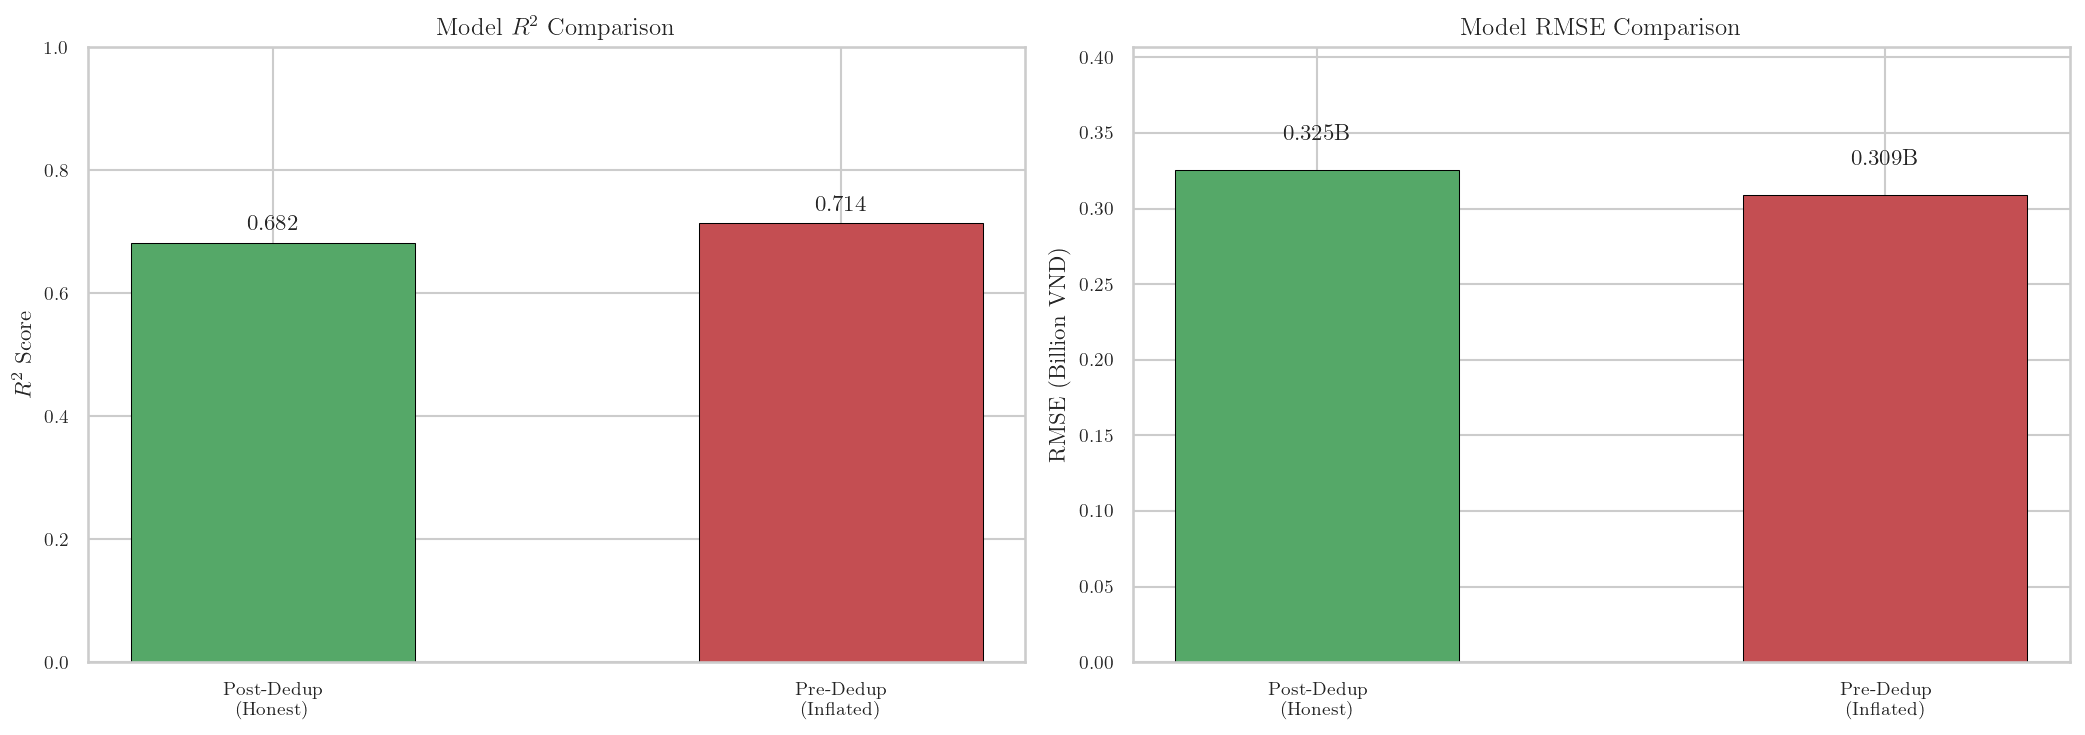
\includegraphics[width=\textwidth]{before_after_comparison}
\caption{Model performance before and after data quality corrections. The
``before'' metrics were inflated by duplicate-induced test--train leakage.}
\label{fig:before_after}
\end{figure*}

\subsection{Impact Summary}
Table~\ref{tab:quality_impact} quantifies the cumulative impact of each
data quality fix.

\begin{table}[!t]
\caption{Impact of Data Quality Corrections\label{tab:quality_impact}}
\centering
\begin{tabular}{lrr}
\toprule
\textbf{Stage} & \textbf{Records} & \textbf{Best RMSE} \\
\midrule
Raw (with all issues) & 3,992 & 1.02B VND \\
+ chotot.com price fix & 3,992 & -- \\
+ Deduplication & 3,105 & -- \\
+ BYD removal & 3,015 & 332M VND \\
\bottomrule
\end{tabular}
\end{table}

% ============================================================================
\section{Feature Engineering}

After data cleaning, we engineered 41 features from the remaining 3,015
records through imputation, derivation, EV specification recovery, and a
hybrid encoding strategy.

\subsection{Missing Value Imputation}
Domain-informed imputation was applied to four columns:
\begin{itemize}
    \item \textbf{Brand} (27 NaN): imputed via base\_model$\to$brand lookup
    (all missing-brand records were identifiable VinFast models).
    \item \textbf{Year} (67 NaN): median year per base\_model, with global
    median fallback.
    \item \textbf{Condition}: rule-based---mileage$= 0$ and year$\geq 2025$
    implies ``New''; otherwise ``Used.''
    \item \textbf{Mileage} (281 NaN): 0~km for new cars; median per brand
    for used cars. Values exceeding 300,000~km were treated as outliers and
    re-imputed with the per-brand median.
\end{itemize}

Vietnamese categorical values (drivetrain, origin, exterior color, city) were
mapped to English equivalents for consistent encoding.

\subsection{Derived Features}
Three numeric features were derived:
\begin{itemize}
    \item $\texttt{car\_age} = 2026 - \texttt{year}$ (depreciation proxy)
    \item $\texttt{log\_mileage} = \log(1 + \texttt{mileage\_km})$ (reduces
    right skew)
    \item $\texttt{is\_new} \in \{0, 1\}$ (binary condition indicator)
\end{itemize}

\subsection{EV Specifications Recovery}
One of the most impactful feature engineering steps was recovering
EV-specific technical specifications. The otodien.vn source dataset contained
battery capacity (kWh), driving range (km), and motor power (hp) for 728
records with 99.6\% fill rate. We constructed a lookup table mapping each
base\_model to its median battery\_kwh, range\_km, and power\_hp, yielding
specifications for 29 distinct EV models. This lookup was then joined to all
records.

These three features capture the fundamental physics of EV pricing: a VinFast
VF3 with 18.6~kWh battery and 210~km range is priced around 315M~VND, while
a VF9 with 92~kWh and 480~km range commands approximately 1.5B~VND.
Fig.~\ref{fig:ev_specs} shows the specification distribution across models.

\begin{figure*}[!t]
\centering
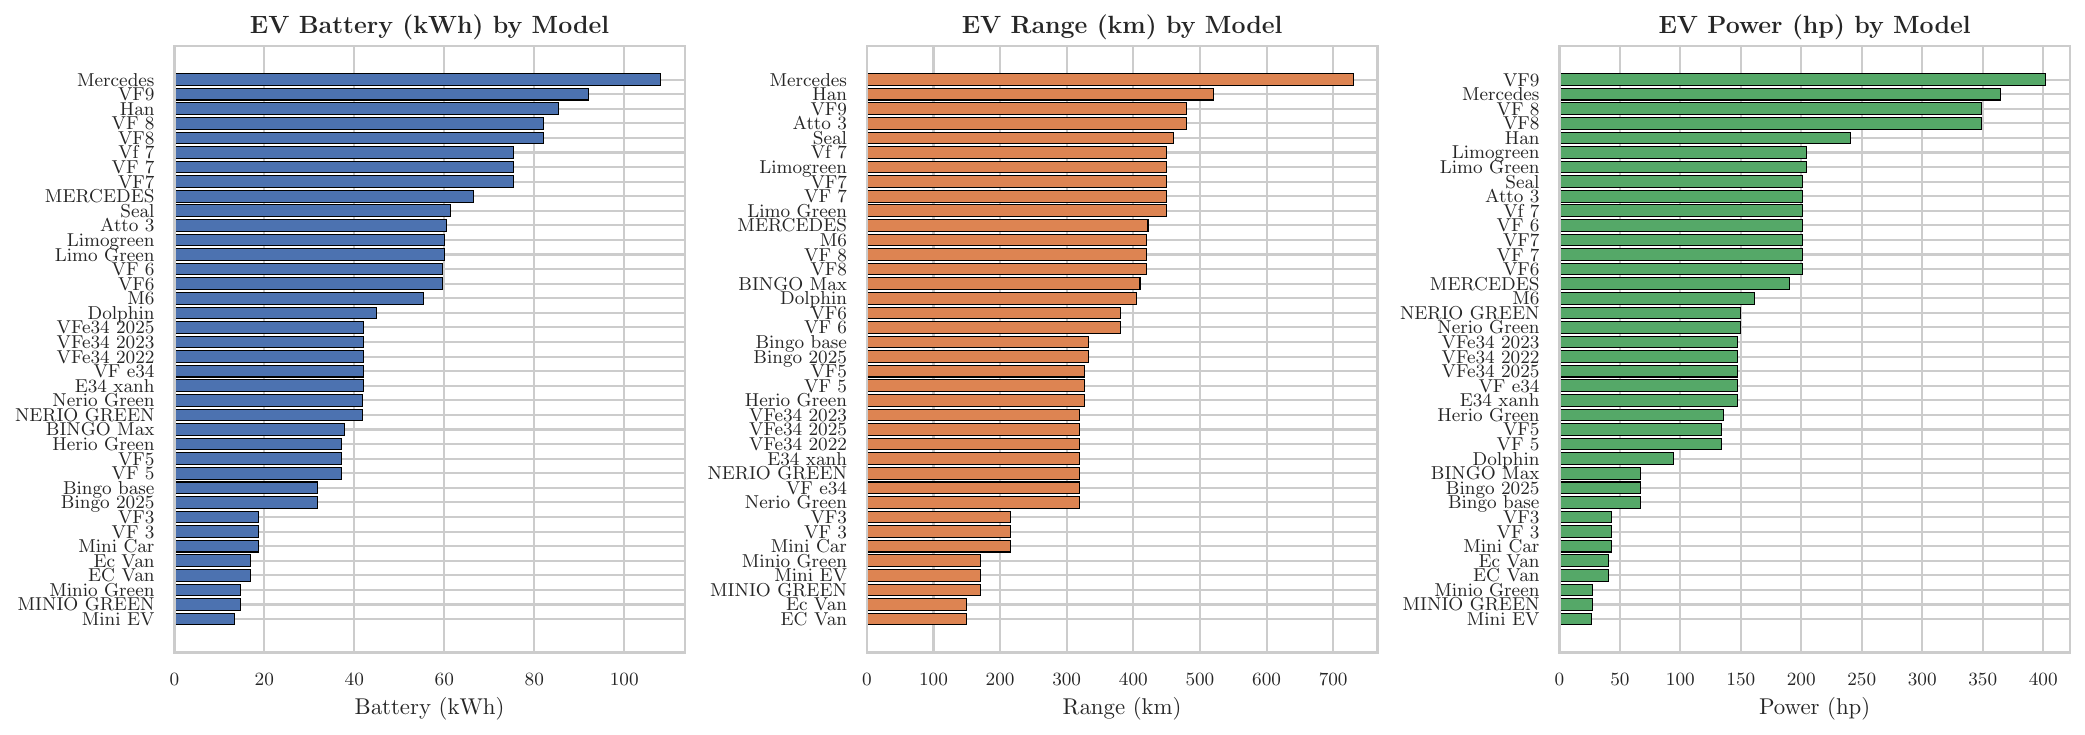
\includegraphics[width=\textwidth]{ev_specs_coverage}
\caption{EV specifications (battery capacity, range, power) across models in
the lookup table.}
\label{fig:ev_specs}
\end{figure*}

\subsection{Encoding Strategy}
We adopted a hybrid encoding strategy after an important negative result:
\textit{target-encoding all categorical features caused $R^2$ to drop from
0.79 to 0.087.} The root cause was that target-encoded features for the
dominant brand (VinFast, 93.6\% of data) converged to a near-constant value
($\sim$2.6B~VND mean), despite actual VinFast prices ranging from
50M--14B~VND. The model became ``lazy,'' relying solely on the brand
encoding.

Our solution:
\begin{itemize}
    \item \textbf{Target encoding} (leave-one-out with Bayesian smoothing,
    $m=10$) for high-cardinality features only: \texttt{model\_mode} (324
    unique values, Pearson $r = 0.76$ between its encoded values and price) and \texttt{model\_year}
    (interaction of base\_model and year).
    \item \textbf{One-hot encoding} for low-cardinality features: brand
    ($\leq 8$), base\_model ($\sim$15), body\_type (5), drivetrain (3),
    origin (3). Rare categories ($< 10$ records) were grouped into ``Other.''
    \item \textbf{Dropped}: exterior\_color, city, brand\_body (low signal
    after EV specs were added).
\end{itemize}

The leave-one-out target encoding formula with Bayesian smoothing is:
\begin{equation}
\hat{y}_i = \frac{n_c \cdot \bar{y}_c + m \cdot \bar{y}_{\text{global}}}{n_c + m}
\label{eq:target_enc}
\end{equation}
where $n_c$ is the category count, $\bar{y}_c$ is the category mean, and
$m = 10$ is the smoothing parameter. During training, each observation's
own value is excluded from the category mean to prevent leakage.

Fig.~\ref{fig:encoding} and Fig.~\ref{fig:feature_importance} show the
encoding strategy and resulting feature importance.

\begin{figure}[!t]
\centering
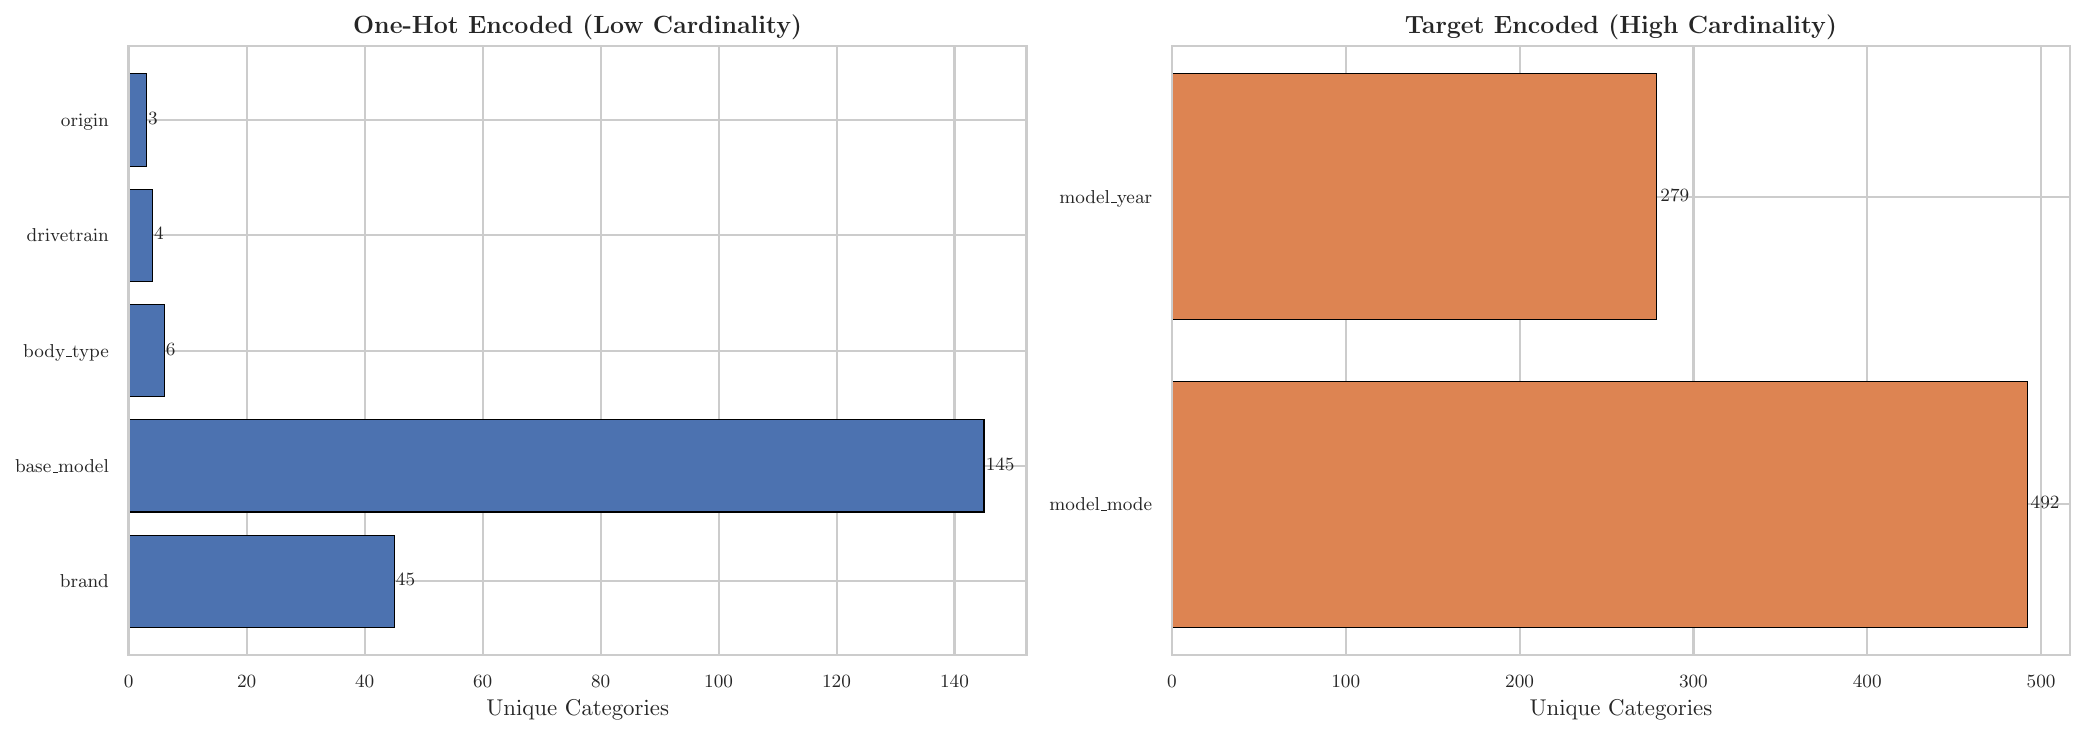
\includegraphics[width=\columnwidth]{encoding_comparison}
\caption{Hybrid encoding strategy: one-hot for low cardinality (left),
target encoding for high cardinality (right).}
\label{fig:encoding}
\end{figure}

\begin{figure*}[!t]
\centering
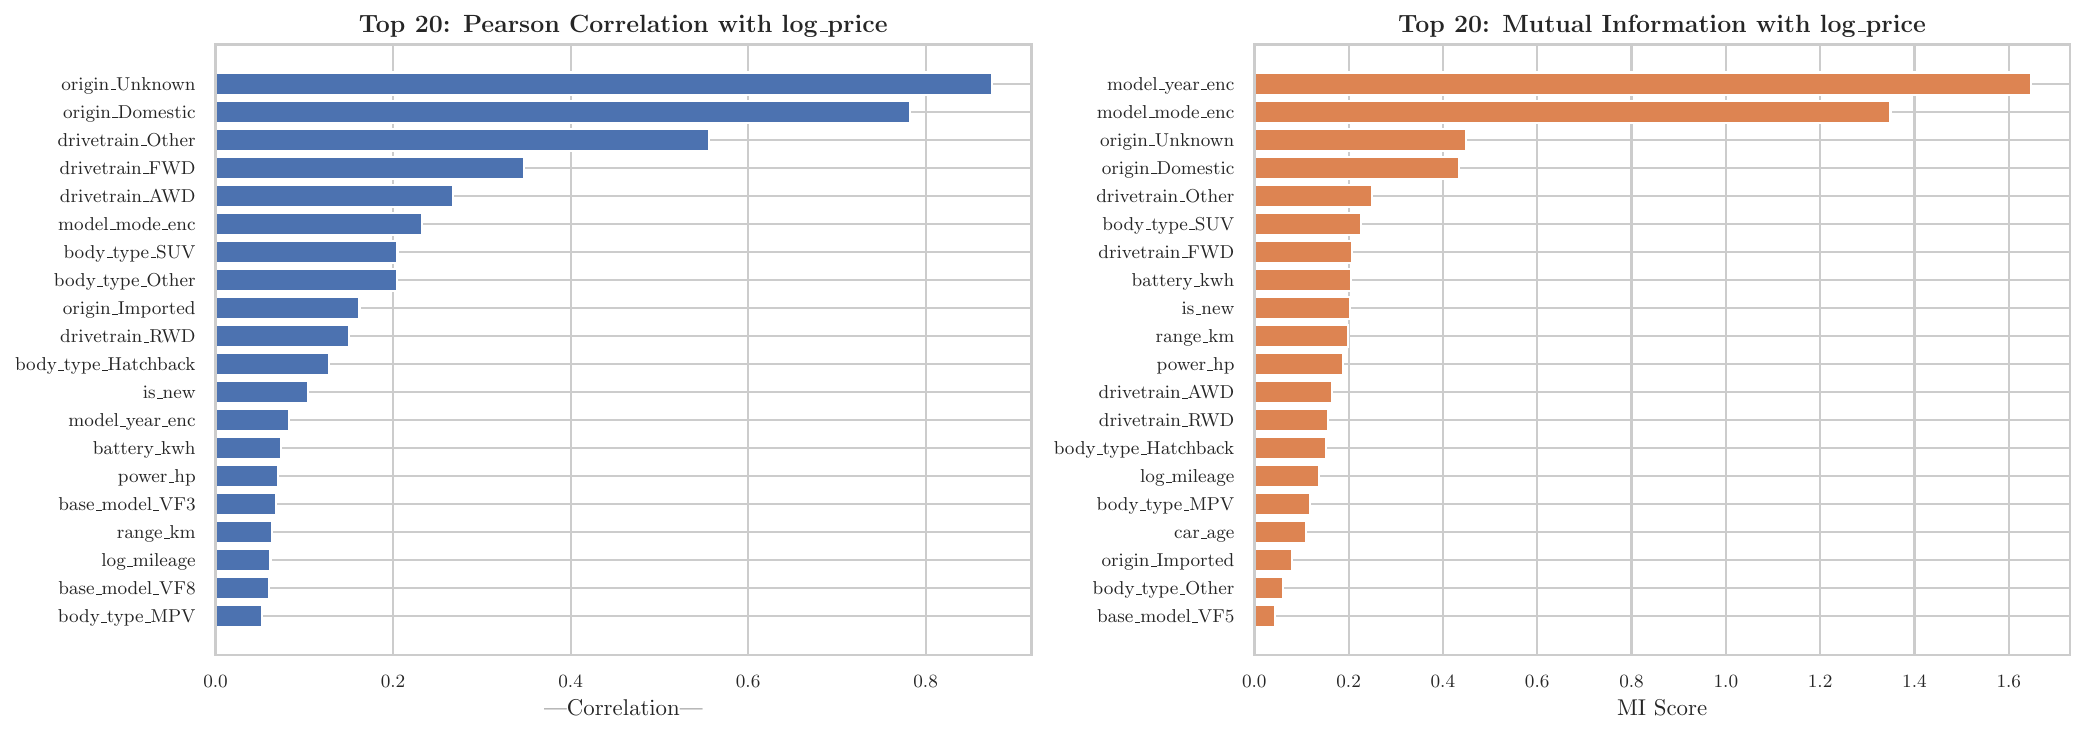
\includegraphics[width=\textwidth]{feature_importance_summary}
\caption{Top 20 features ranked by Pearson correlation (left) and mutual
information (right) with log-transformed price.}
\label{fig:feature_importance}
\end{figure*}

Table~\ref{tab:features} summarizes the final feature set.

\begin{table}[!t]
\caption{Final Feature Set (41 Features)\label{tab:features}}
\centering
\begin{tabular}{llr}
\toprule
\textbf{Category} & \textbf{Features} & \textbf{Count} \\
\midrule
Numeric & car\_age, log\_mileage, is\_new, & 4 \\
 & has\_aftermarket\_mods & \\
EV Specifications & battery\_kwh, range\_km, power\_hp & 3 \\
Target-Encoded & model\_mode\_enc, model\_year\_enc & 2 \\
One-Hot: Brand & VinFast, Porsche, Mercedes, \ldots & 5 \\
One-Hot: Model & VF3, VF5, VF6, VF7, VF8, VF9, \ldots & 15 \\
One-Hot: Body & SUV, Hatchback, MPV, Sedan, \ldots & 5 \\
One-Hot: Drive & AWD, FWD, RWD & 3 \\
One-Hot: Origin & Domestic, Imported, Unknown & 3 \\
\midrule
\multicolumn{2}{l}{\textbf{Total}} & \textbf{41} \\
\bottomrule
\end{tabular}
\end{table}

% ============================================================================
\section{Experimental Setup}

\subsection{Train--Test Split}
The cleaned dataset (3,015 records) was split 80/20 into training (2,412)
and test (603) sets, stratified on \texttt{base\_model}. Stratification on
base\_model is more informative than on brand in this dataset, where 93.6\%
of records belong to VinFast. Rare models ($< 5$ records) were grouped for
stratification purposes. Sample weights based on inverse quintile frequency
of the target-encoded base\_model were computed to mitigate brand
concentration bias during training.

\subsection{Models}
We benchmarked four regression models representing different paradigms:
\begin{itemize}
    \item \textbf{Ridge Regression}: $L_2$-regularized linear model trained
    on standardized features with log-transformed target.
    \item \textbf{Support Vector Regression (SVR)}: RBF kernel on
    standardized features with log-transformed target.
    \item \textbf{Random Forest}: Ensemble (300--600 trees, grid-searched)
    on unscaled features with raw price target.
    \item \textbf{XGBoost}: Gradient-boosted trees on unscaled features with
    raw price target.
\end{itemize}

Ridge and SVR use log-transformed targets and standardized features to
handle the heavy right-skew of Vietnamese EV prices (skewness = 5.03 for
raw prices, 0.22 for log-transformed). Tree-based models operate on raw
prices and unscaled features, leveraging their inherent invariance to
monotonic transformations.

\subsection{Hyperparameter Tuning}
All models were tuned via 5-fold cross-validation using GridSearchCV. The
search grids were designed for the dataset characteristics (2,412 training
rows, 41 features):
\begin{itemize}
    \item Ridge: $\alpha \in \{0.001, 0.01, 0.1, 1, 10, 100\}$
    \item SVR: $C \in \{1, 10, 100, 1000\}$, $\epsilon \in \{0.001, 0.01, 0.1\}$,
    $\gamma \in \{\text{scale}, \text{auto}\}$
    \item RF: $n_{\text{est}} \in \{300, 600\}$, max\_depth $\in \{10, 20, \text{None}\}$,
    max\_features $\in \{\sqrt{}, 0.5, 0.8\}$
    \item XGBoost: $n_{\text{est}} \in \{300, 600\}$, max\_depth $\in \{4, 8, 12\}$,
    learning\_rate $\in \{0.01, 0.05, 0.1\}$, subsample $\in \{0.8, 1.0\}$,
    colsample\_bytree $\in \{0.8, 1.0\}$, min\_child\_weight $\in \{3, 5\}$
\end{itemize}

\subsection{Evaluation Metrics}
We report RMSE, MAE, $R^2$, adjusted $R^2$, and MAPE on the held-out test
set. Additionally, we introduce segment-specific evaluation using four price
tiers reflecting the Vietnamese EV market structure:
\begin{itemize}
    \item \textbf{Budget}: $< 500$M VND (entry-level EVs)
    \item \textbf{Mid}: 500M--1.2B VND (family EVs)
    \item \textbf{Premium}: 1.2B--5B VND (high-end domestic)
    \item \textbf{Luxury}: $> 5$B VND (imported luxury)
\end{itemize}

% ============================================================================
\section{Results and Discussion}

\subsection{Overall Benchmark}
Table~\ref{tab:benchmark} presents the test-set performance of all four
models after hyperparameter tuning on the cleaned dataset.

\begin{table}[!t]
\caption{Model Benchmark Results on Test Set ($n = 603$)\label{tab:benchmark}}
\centering
\begin{tabular}{lrrrrr}
\toprule
\textbf{Model} & \textbf{RMSE} & \textbf{MAE} & \textbf{$R^2$} & \textbf{Adj.\ $R^2$} & \textbf{MAPE} \\
 & (M VND) & (M VND) & & & (\%) \\
\midrule
Ridge & 381 & 115 & 0.636 & 0.610 & 43.5 \\
SVR & 369 & 94 & 0.660 & 0.635 & 48.9 \\
\textbf{Random Forest} & \textbf{332} & \textbf{89} & \textbf{0.725} & \textbf{0.705} & \textbf{43.6} \\
XGBoost & 383 & 103 & 0.633 & 0.606 & 43.0 \\
\bottomrule
\end{tabular}
\end{table}

Random Forest achieved the best performance across all metrics, with RMSE of
332M~VND and $R^2 = 0.725$. The 95\% confidence interval for RF RMSE is
[139M, 496M]~VND, computed via bootstrap resampling. The tree-based models
(RF and XGBoost) and SVR significantly outperformed Ridge Regression in MAE,
suggesting that non-linear relationships between features and price are
important.

Fig.~\ref{fig:model_rmse} and Fig.~\ref{fig:model_r2} compare the models
visually.

\begin{figure}[!t]
\centering
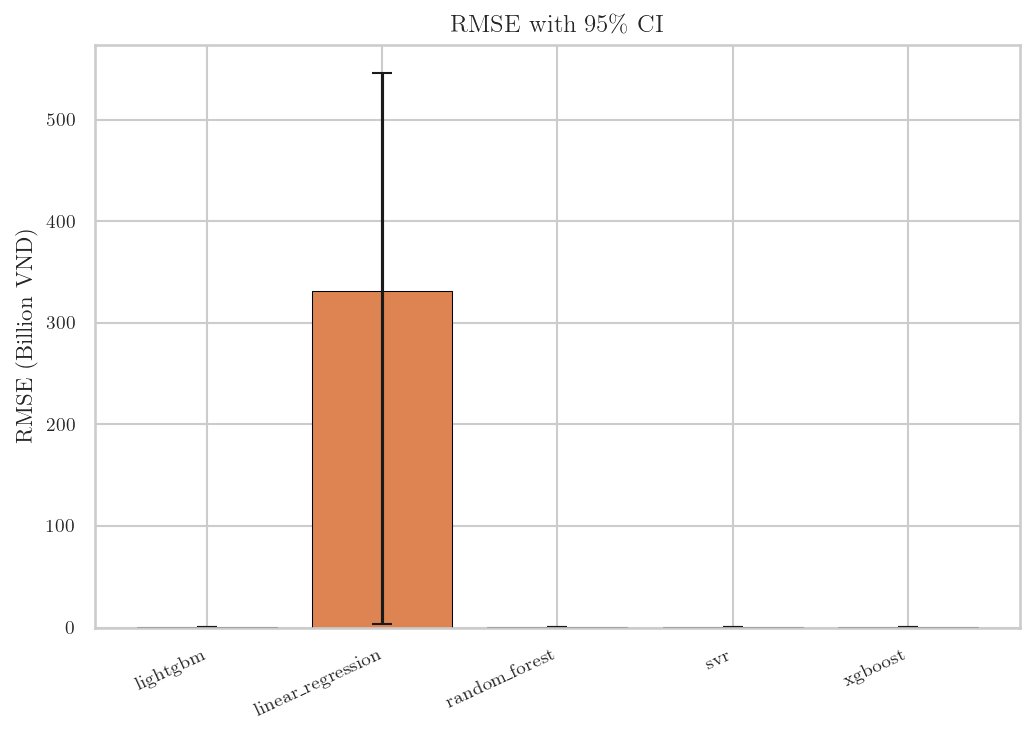
\includegraphics[width=\columnwidth]{model_rmse_comparison}
\caption{RMSE comparison across four regression models.}
\label{fig:model_rmse}
\end{figure}

\begin{figure}[!t]
\centering
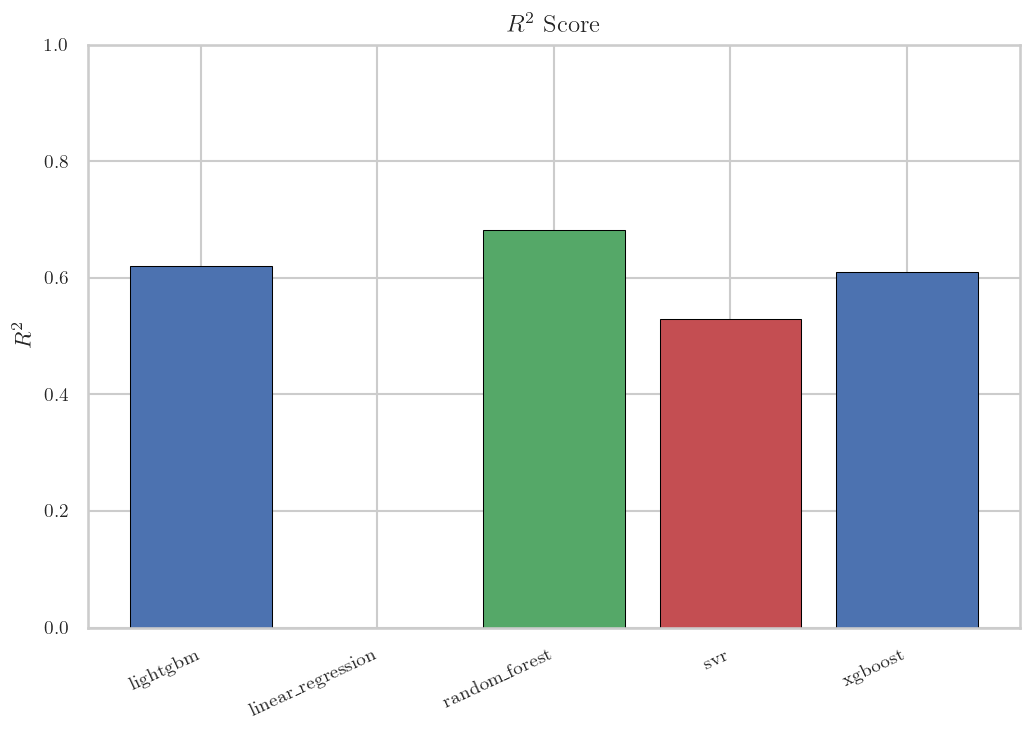
\includegraphics[width=\columnwidth]{model_r2_comparison}
\caption{$R^2$ comparison across four regression models.}
\label{fig:model_r2}
\end{figure}

\subsection{Segment-Specific Analysis}
Table~\ref{tab:segments} reveals substantial performance variation across
price segments for the best model (Random Forest).

\begin{table}[!t]
\caption{Random Forest Performance by Price Segment\label{tab:segments}}
\centering
\begin{tabular}{lrrr}
\toprule
\textbf{Segment} & \textbf{$n$ (test)} & \textbf{RMSE (M VND)} & \textbf{MAE (M VND)} \\
\midrule
Budget ($< 500$M) & 237 & 100 & 45 \\
Mid (500M--1.2B) & 318 & 81 & 58 \\
Premium (1.2B--5B) & 46 & 797 & 394 \\
Luxury ($> 5$B) & 2 & 4,041 & 3,275 \\
\midrule
\textbf{Overall} & \textbf{603} & \textbf{332} & \textbf{89} \\
\bottomrule
\end{tabular}
\end{table}

The budget and mid-range segments---comprising 92\% of test records (555 of
603)---achieve RMSE of 100M and 81M~VND respectively, representing
prediction errors of approximately 34\% and 11\% of median segment price.
These error levels are practical for price estimation on the scraped
websites. The premium segment (RMSE = 797M) and luxury segment (RMSE = 4B,
$n = 2$) remain impractical due to sparse data and high price variance.

Fig.~\ref{fig:segment_rmse} visualizes the segment-level RMSE across all
four models.

\begin{figure}[!t]
\centering
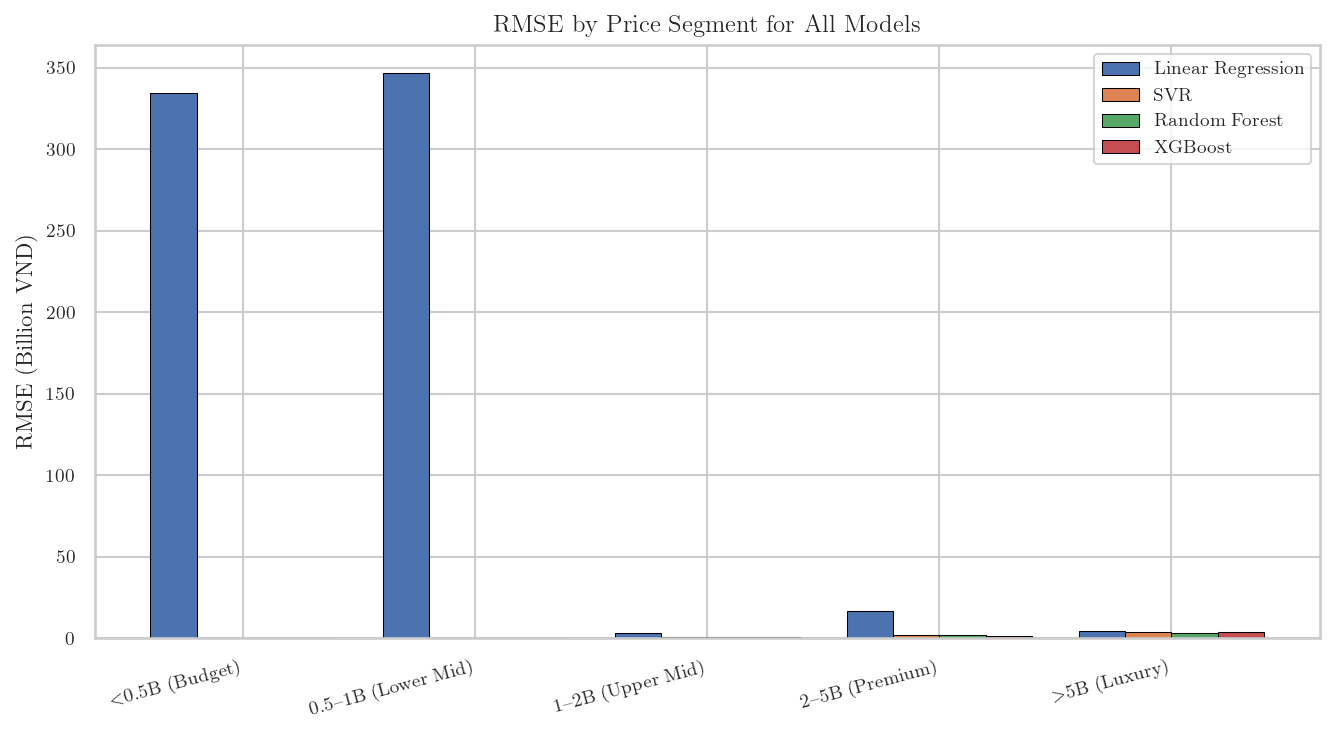
\includegraphics[width=\columnwidth]{segment_rmse}
\caption{RMSE by price segment for all four models. Budget and mid segments
show practical accuracy; luxury is dominated by data sparsity.}
\label{fig:segment_rmse}
\end{figure}

\subsection{Feature Importance}
Fig.~\ref{fig:rf_importance} shows the Random Forest permutation feature
importance. The target-encoded \texttt{model\_mode\_enc} (trim level) is the
most important feature, confirming our decision to recover this
high-correlation ($r = 0.76$) signal via target encoding rather than
discarding it due to high cardinality. The EV specification features
(battery\_kwh, range\_km, power\_hp) rank among the top predictors, validating
the lookup-table recovery approach.

\begin{figure}[!t]
\centering
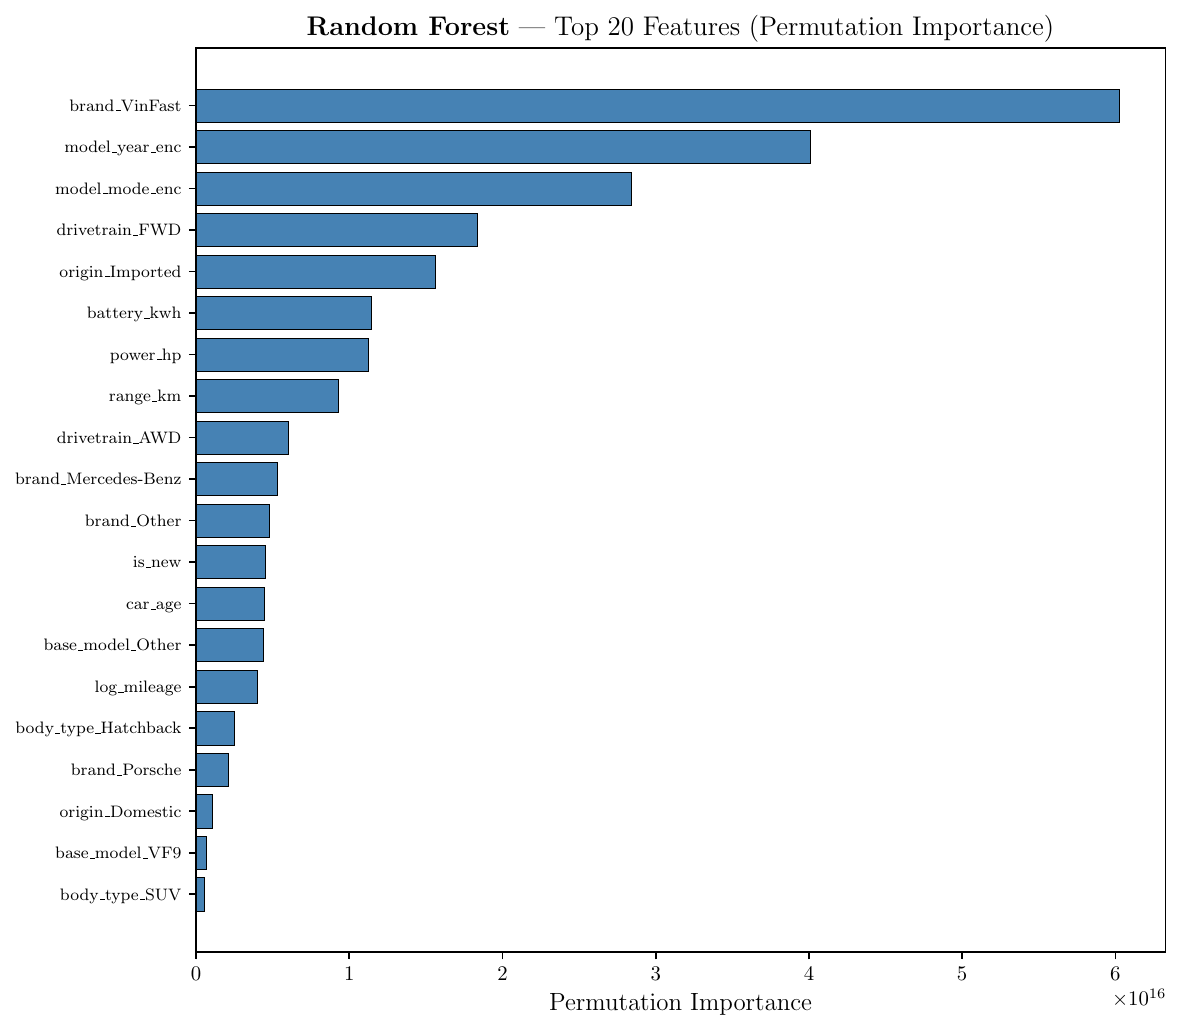
\includegraphics[width=\columnwidth]{random_forest_feature_importance}
\caption{Random Forest feature importance (top 20 features).}
\label{fig:rf_importance}
\end{figure}

\subsection{Residual Analysis}
Fig.~\ref{fig:rf_pred} shows the actual versus predicted scatter for Random
Forest. Predictions cluster well along the diagonal for prices below
1.5B~VND, with increasing dispersion for higher-priced vehicles.
Fig.~\ref{fig:rf_residuals} shows the residual distribution, which is
approximately symmetric around zero with heavy tails driven by the premium
and luxury segments.

\begin{figure}[!t]
\centering
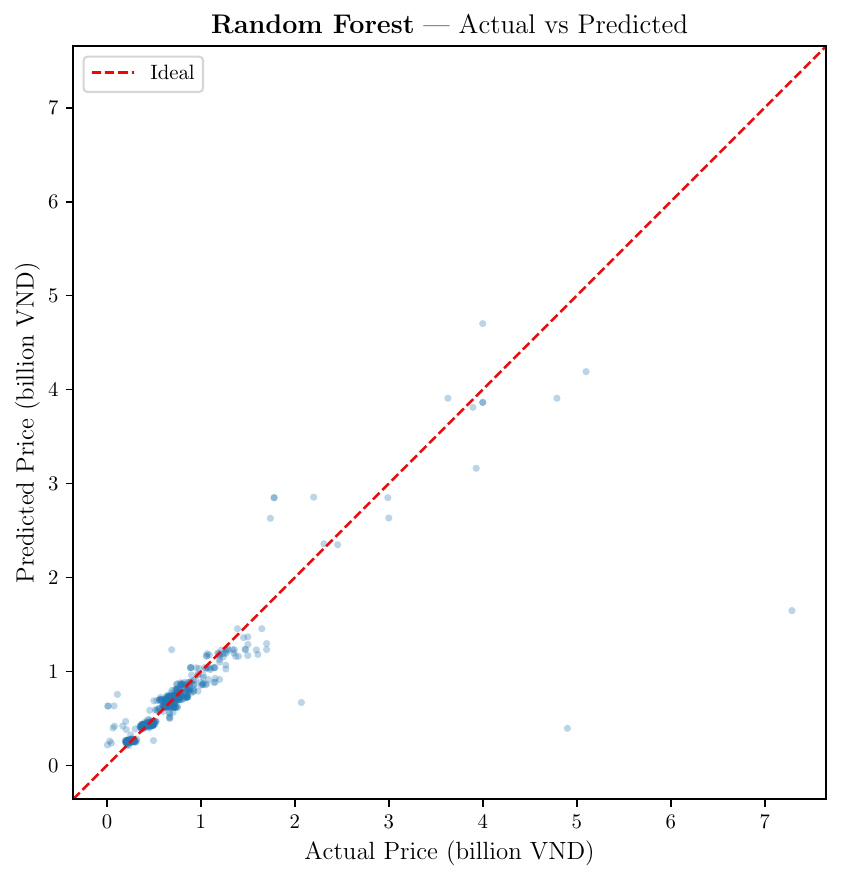
\includegraphics[width=\columnwidth]{random_forest_actual_vs_predicted}
\caption{Actual versus predicted prices for Random Forest. Points near the
diagonal indicate accurate predictions.}
\label{fig:rf_pred}
\end{figure}

\begin{figure}[!t]
\centering
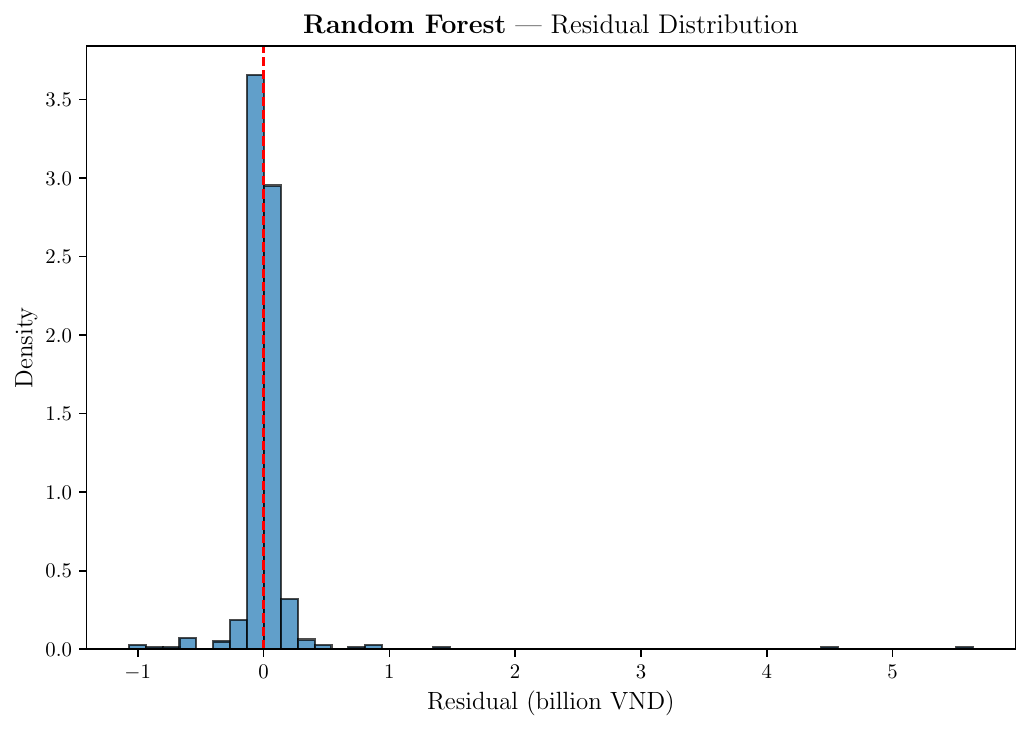
\includegraphics[width=\columnwidth]{random_forest_residual_distribution}
\caption{Distribution of prediction residuals for Random Forest.}
\label{fig:rf_residuals}
\end{figure}

\subsection{Data Quality vs.\ Model Selection}
A key finding of this study is the relative importance of data quality
remediation versus model architecture. The data quality corrections (chotot.com
price fix, deduplication, BYD removal) reduced RMSE from 1.02B to 332M~VND---a
67\% improvement. By contrast, the difference between the best (RF, 332M) and
worst (XGBoost, 383M) models on the cleaned data is only 51M~VND (15\%). This
suggests that in real-world applied ML settings where data is scraped rather
than curated, investment in data quality analysis yields substantially higher
returns than model experimentation.

% ============================================================================
\section{Limitations and Future Work}

Several limitations constrain the generalizability of our results:

\textbf{Brand concentration.} VinFast accounts for 93.6\% of all records,
reflecting the actual market composition but limiting the model's ability to
price non-VinFast vehicles accurately.

\textbf{Dataset size.} At 3,015 clean records (2,412 training), the dataset
is small by modern ML standards. This particularly affects the premium and
luxury segments, where $n < 50$ in the test set.

\textbf{No temporal modeling.} All listings are treated as cross-sectional.
The model does not account for time-varying factors such as depreciation
curves, seasonal demand, or policy changes (e.g., EV subsidies).

\textbf{Luxury segment.} With only 2 test records in the luxury segment, the
4B~VND RMSE is statistically unreliable and practically useless.

Future work could address these limitations through: (1)~continuous scraping
to build a time-series dataset for depreciation modeling; (2)~incorporating
additional data sources (official dealer prices, government registration
data); (3)~ensemble stacking of the four models; (4)~expanding to hybrid and
plug-in hybrid vehicles as the Vietnamese market diversifies.

% ============================================================================
\section{Conclusion}

We presented an end-to-end pipeline for electric vehicle price prediction in
the Vietnamese market, spanning web scraping, LLM-assisted feature
extraction, data quality analysis, feature engineering, and regression
benchmarking. Our primary finding is that systematic data quality
remediation---identifying and correcting a 10$\times$ source-level price
inflation, removing systematically erroneous brand data, and eliminating
duplicate-induced test--train leakage---reduced RMSE by 67\%, from 1.02B to
332M~VND. This improvement far exceeds the gains from model selection
(15\% difference between best and worst models on clean data).

Random Forest achieved the best overall performance ($R^2 = 0.725$,
RMSE = 332M~VND), with practical accuracy in the budget ($< 500$M, RMSE =
100M) and mid-range (500M--1.2B, RMSE = 81M) segments that constitute the
majority of the Vietnamese EV market. The target-encoded trim level
(\texttt{model\_mode\_enc}) and recovered EV specifications (battery
capacity, range, power) emerged as the most predictive features, confirming
that domain-specific feature recovery is essential for EV pricing.

Our work demonstrates that in applied ML settings with web-scraped data,
the dominant bottleneck is data quality, not model architecture---a finding
with broad implications for practitioners constructing ML pipelines from
real-world internet data.

% ============================================================================
%\section*{Acknowledgments}
%[To be added by authors.]

% ============================================================================
\begin{thebibliography}{20}
\bibliographystyle{IEEEtran}

\bibitem{vn_ev_policy}
Vietnamese Government, ``Decision No.\ 876/QD-TTg: National strategy on
green growth for the period 2021--2030,'' 2021.

\bibitem{gegic2019}
E.~Gegic, B.~Isakovic, D.~Keco, Z.~Masetic, and J.~Kevric, ``Car price
prediction using machine learning techniques,'' \textit{TEM Journal},
vol.~8, no.~1, pp.~113--118, 2019.

\bibitem{vw_price}
A.~Krizhevsky and H.~Mu, ``Used car price prediction using machine
learning techniques,'' in \textit{Proc.\ Int.\ Conf.\ Identification,
Information and Knowledge in the Internet of Things}, 2018.

\bibitem{pal2018}
N.~Pal, P.~Arora, P.~Kohli, D.~Sundararaman, and S.~S.~Palakurthy,
``How much is my car worth? A methodology for predicting used cars' prices
using random forest,'' in \textit{Proc.\ Future of Information and
Communication Conf.}, Springer, 2018, pp.~413--422.

\bibitem{pudaruth2014}
S.~Pudaruth, ``Predicting the price of used cars using machine learning
techniques,'' \textit{Int.\ J.\ Inf.\ Comput.\ Technol.}, vol.~4, no.~7,
pp.~753--764, 2014.

\bibitem{hedonic_pricing}
S.~Rosen, ``Hedonic prices and implicit markets: Product differentiation in
pure competition,'' \textit{J.\ Political Economy}, vol.~82, no.~1,
pp.~34--55, 1974.

\bibitem{mitchell_scraping}
R.~Mitchell, \textit{Web Scraping with Python}, 2nd ed.\ O'Reilly Media,
2018.

\bibitem{lessmann2019}
S.~Lessmann, B.~Baesens, H.~V.~Seow, and L.~C.~Thomas, ``Benchmarking
state-of-the-art classification algorithms for credit scoring: An update
of research,'' \textit{European J.\ Operational Research}, vol.~247, no.~1,
pp.~124--136, 2015.

\bibitem{wei2023}
J.~Wei, X.~Wang, D.~Schuurmans, M.~Bosma, E.~Chi, Q.~Le, and D.~Zhou,
``Chain-of-thought prompting elicits reasoning in large language models,''
in \textit{Proc.\ NeurIPS}, 2022.

\bibitem{ollama2024}
Ollama, ``Run large language models locally,'' 2024. [Online]. Available:
\url{https://ollama.com/}

\bibitem{bs4}
L.~Richardson, ``Beautiful Soup: HTML/XML parser for Python,'' 2023.
[Online]. Available: \url{https://www.crummy.com/software/BeautifulSoup/}

\bibitem{scrapy}
Scrapy developers, ``Scrapy: A fast high-level web crawling framework,''
2024. [Online]. Available: \url{https://scrapy.org/}

\bibitem{selenium}
Selenium, ``Selenium WebDriver,'' 2024. [Online]. Available:
\url{https://www.selenium.dev/}

\bibitem{sklearn}
F.~Pedregosa \textit{et al.}, ``Scikit-learn: Machine learning in Python,''
\textit{J.\ Mach.\ Learn.\ Res.}, vol.~12, pp.~2825--2830, 2011.

\bibitem{xgboost}
T.~Chen and C.~Guestrin, ``XGBoost: A scalable tree boosting system,'' in
\textit{Proc.\ 22nd ACM SIGKDD Int.\ Conf.\ Knowledge Discovery and Data
Mining}, 2016, pp.~785--794.

\end{thebibliography}

\end{document}
